% \section{Appendix}

% \subsection{Code Base}
\begin{frame}{Appendix 1 - UML for Repository Testing DSL}
\begin{figure}[H]
  \centering
    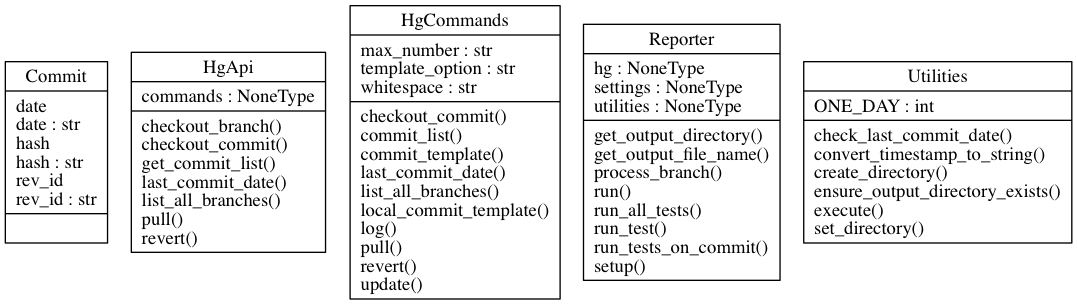
\includegraphics[width=300px]{figures/python_dsl_classes.png}
  \caption{UML Diagram for Repository Testing DSL}
\end{figure}
\end{frame}

% \subsection{Design Patterns}
\begin{frame}{Appendix 2 - Design Patterns}
\begin{itemize}
\item Singleton
\item Factory Pattern
\item Builder Pattern
\item Future Await Pattern
\end{itemize}
\end{frame}

% \subsection{Choice of Configuration Media}
\begin{frame}{Appendix 3 - YAML for configuration}
\textbf{YAML} was chosen as the markup language for configuration language for the DSLs. An example of the YAML markup is shown below:
\begin{figure}[H]
  \centering
    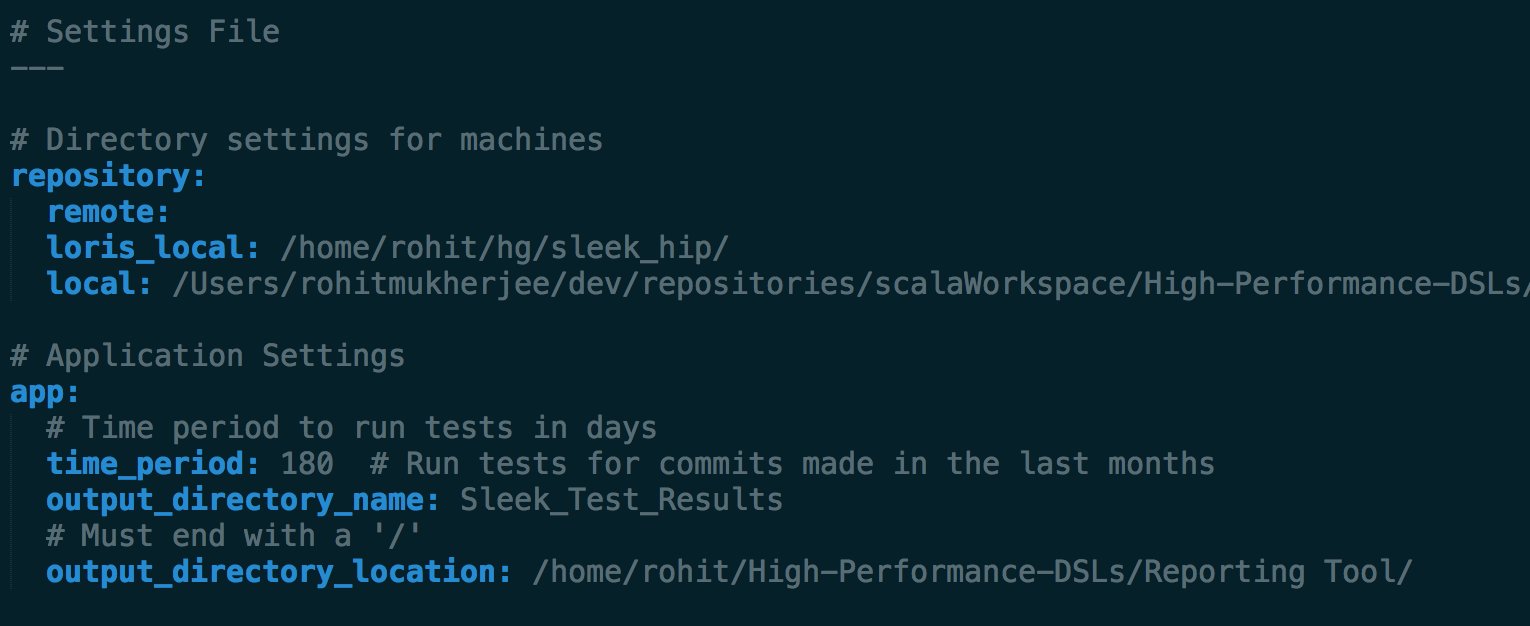
\includegraphics[width=300px]{figures/settings.png}
  \caption{settings.yaml - used to configure the reporting tool}
\end{figure}
\end{frame}

\begin{frame}{Appendix 4 - Reasons for choosing YAML}
\begin{itemize}
\item Human Readability (more so than XML/JSON)
\item Low number of format characters
\item Language agnostic, can be parsed easily by different languages
\item Sufficient types of data structures
\item Not verbose like XML
\item Faster than XML
\item Python - like syntax
\end{itemize}
\end{frame}

\begin{frame}{Appendix 5 - Reasons for choosing sbt as build tool}
    \begin{itemize}
    \item Incremental compilation
    \item Interactive Shell
    \item Native support for compiling Scala code and integrating with many Scala test frameworks
    \item Build descriptions written in a Scala DSL\cite{sbt}
    \item Dependency Resolution
    \end{itemize}
\end{frame}